\documentclass{beamer}\usepackage[]{graphicx}\usepackage[]{color}
%% maxwidth is the original width if it is less than linewidth
%% otherwise use linewidth (to make sure the graphics do not exceed the margin)
\makeatletter
\def\maxwidth{ %
  \ifdim\Gin@nat@width>\linewidth
    \linewidth
  \else
    \Gin@nat@width
  \fi
}
\makeatother

\definecolor{fgcolor}{rgb}{0.345, 0.345, 0.345}
\newcommand{\hlnum}[1]{\textcolor[rgb]{0.686,0.059,0.569}{#1}}%
\newcommand{\hlstr}[1]{\textcolor[rgb]{0.192,0.494,0.8}{#1}}%
\newcommand{\hlcom}[1]{\textcolor[rgb]{0.678,0.584,0.686}{\textit{#1}}}%
\newcommand{\hlopt}[1]{\textcolor[rgb]{0,0,0}{#1}}%
\newcommand{\hlstd}[1]{\textcolor[rgb]{0.345,0.345,0.345}{#1}}%
\newcommand{\hlkwa}[1]{\textcolor[rgb]{0.161,0.373,0.58}{\textbf{#1}}}%
\newcommand{\hlkwb}[1]{\textcolor[rgb]{0.69,0.353,0.396}{#1}}%
\newcommand{\hlkwc}[1]{\textcolor[rgb]{0.333,0.667,0.333}{#1}}%
\newcommand{\hlkwd}[1]{\textcolor[rgb]{0.737,0.353,0.396}{\textbf{#1}}}%

\usepackage{framed}
\makeatletter
\newenvironment{kframe}{%
 \def\at@end@of@kframe{}%
 \ifinner\ifhmode%
  \def\at@end@of@kframe{\end{minipage}}%
  \begin{minipage}{\columnwidth}%
 \fi\fi%
 \def\FrameCommand##1{\hskip\@totalleftmargin \hskip-\fboxsep
 \colorbox{shadecolor}{##1}\hskip-\fboxsep
     % There is no \\@totalrightmargin, so:
     \hskip-\linewidth \hskip-\@totalleftmargin \hskip\columnwidth}%
 \MakeFramed {\advance\hsize-\width
   \@totalleftmargin\z@ \linewidth\hsize
   \@setminipage}}%
 {\par\unskip\endMakeFramed%
 \at@end@of@kframe}
\makeatother

\definecolor{shadecolor}{rgb}{.97, .97, .97}
\definecolor{messagecolor}{rgb}{0, 0, 0}
\definecolor{warningcolor}{rgb}{1, 0, 1}
\definecolor{errorcolor}{rgb}{1, 0, 0}
\newenvironment{knitrout}{}{} % an empty environment to be redefined in TeX

\usepackage{alltt}
\usetheme{metropolis}           % Use metropolis theme
\usepackage[utf8]{inputenc}
\usepackage{amsfonts}
\usepackage{amsmath}
\usepackage{natbib}
\usepackage{graphicx}
\usepackage{array,booktabs,tabularx}
\usepackage{epstopdf}
\usepackage{colortbl, xcolor}


\title{AmyloGram:a novel predictor of amyloidogenicity}
\date{}
\author{Micha\l{} Burdukiewicz\inst{1}, Piotr Sobczyk\inst{2}, Stefan R\"{o}diger\inst{3}, Pawe\l{} Mackiewicz\inst{1} and Ma\l{}gorzata Kotulska\inst{4}}
\institute{\small{\textsuperscript{1}University of Wroc\l{}aw, Department of Genomics, 

\textsuperscript{2}Wroc\l{}aw University of Science and Technology, Faculty of Pure and Applied Mathematics,

\textsuperscript{3}Brandenburg University of Technology Cottbus-Senftenberg, Institute of Biotechnology, 

\textsuperscript{4}Wroc\l{}aw University of Science and Technology, Department of Biomedical Engineering}}
\IfFileExists{upquote.sty}{\usepackage{upquote}}{}
\begin{document}
  \maketitle
  \section{Amyloids}
  
  \begin{frame}{}

  
  
    Proteins associated with various neurodegenerative disorders (e.g., Alzheimer's, Parkinson'a's, Creutzfeldta-Jakob'a's diseases) creating harmful aggregates.
    
    \begin{figure} 
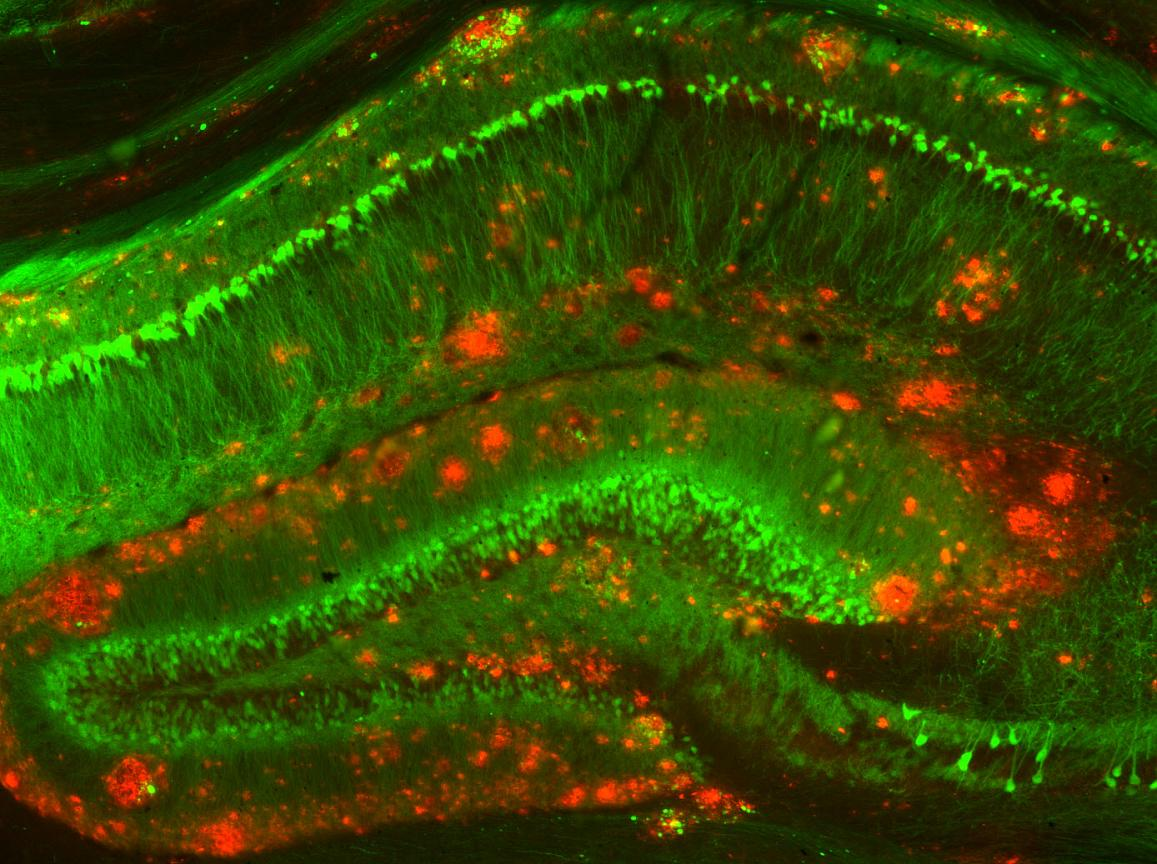
\includegraphics[width=0.85\textwidth]{static_figure/amyloid_aggregates.jpg}
\end{figure}

Amyloid aggregates (red) around neurons (green). Strittmatter Laboratory, Yale University
  \end{frame}
  
  \begin{frame}{}
  
  The aggregation of amyloids is initiated by 6- to 15-residue segments called hot spots, diverse subsequences that form unique zipper-like $\beta$-structures.
\begin{figure} 
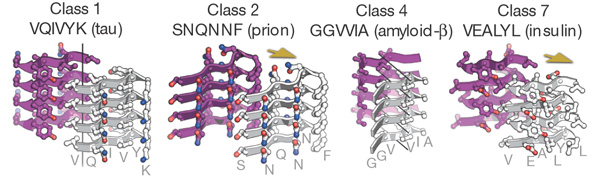
\includegraphics[width=0.55\textwidth]{static_figure/zipper_structure.jpg}
\end{figure}

\citet{sawaya_atomic_2007}
\end{frame}
  
  \begin{frame}{Aim}
  Analize structure of hot spots and create a novel predictor of amyloids.
  \begin{itemize}
  \item Does amyloidogenicity depend on the exact sequence of amino acids?
  \item Which motifs are associated with amyloidogenicity?
  \end{itemize}
  \end{frame}
  
  
\section{Learning framework}  
  
    \begin{frame}{}
\begin{figure} 
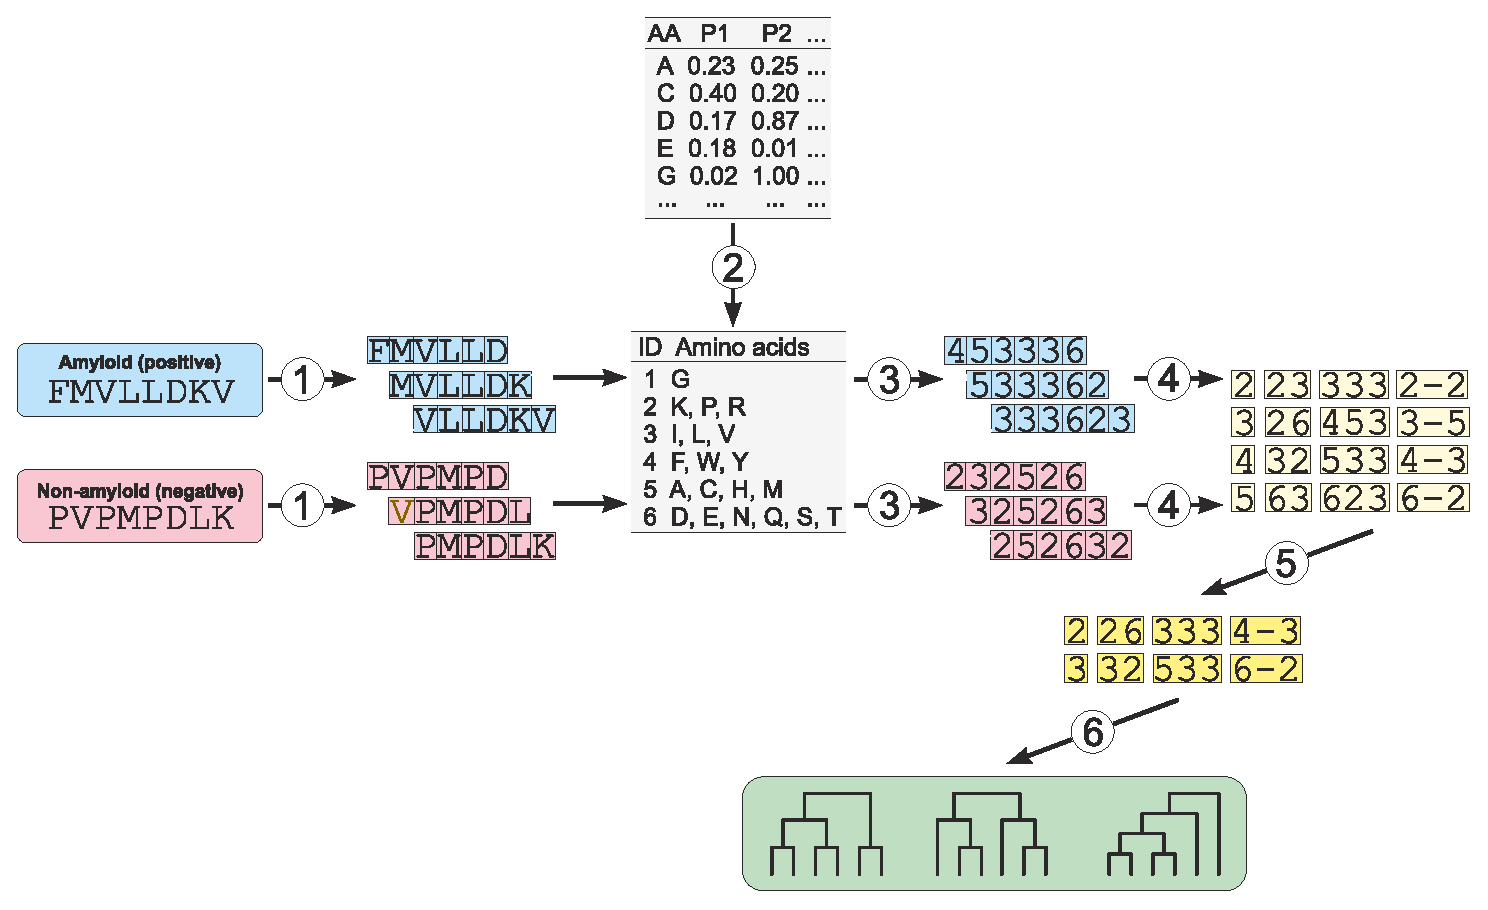
\includegraphics[width=0.95\textwidth]{static_figure/scheme.eps}
\end{figure}

1. Extraction of overlapping hexamers from peptides with known amyloidicity status. 
  \end{frame}

    \begin{frame}{}
\begin{figure} 
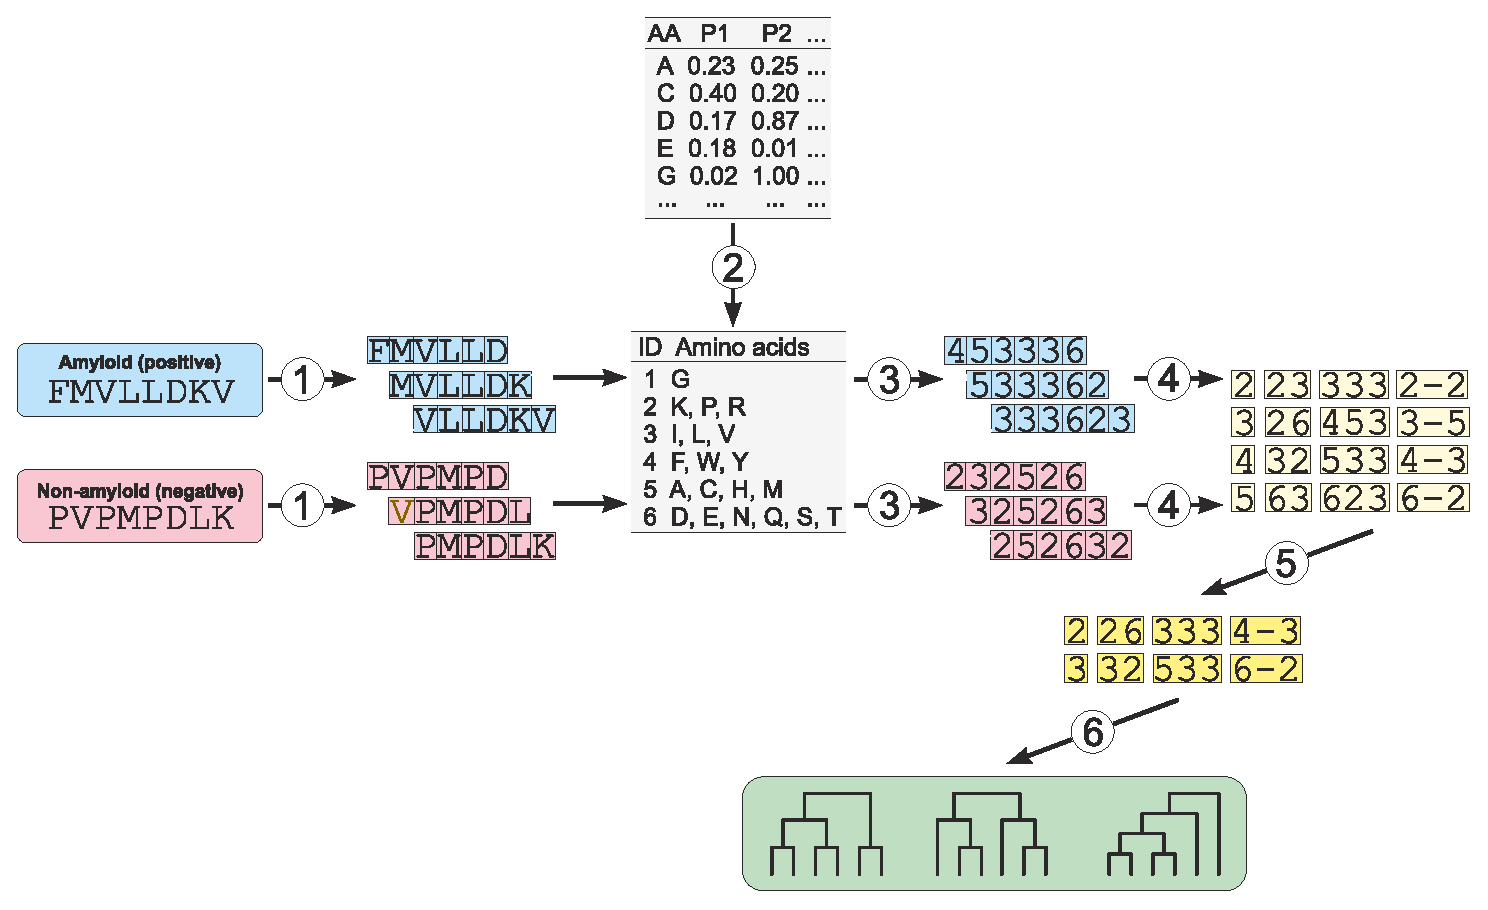
\includegraphics[width=0.95\textwidth]{static_figure/scheme.eps}
\end{figure}

2. Clusterization of amino acids (AA) into groups (ID) using a combination of various 
physicochemical properties (P1, P2, ...).   
\end{frame}

    \begin{frame}{}
\begin{figure} 
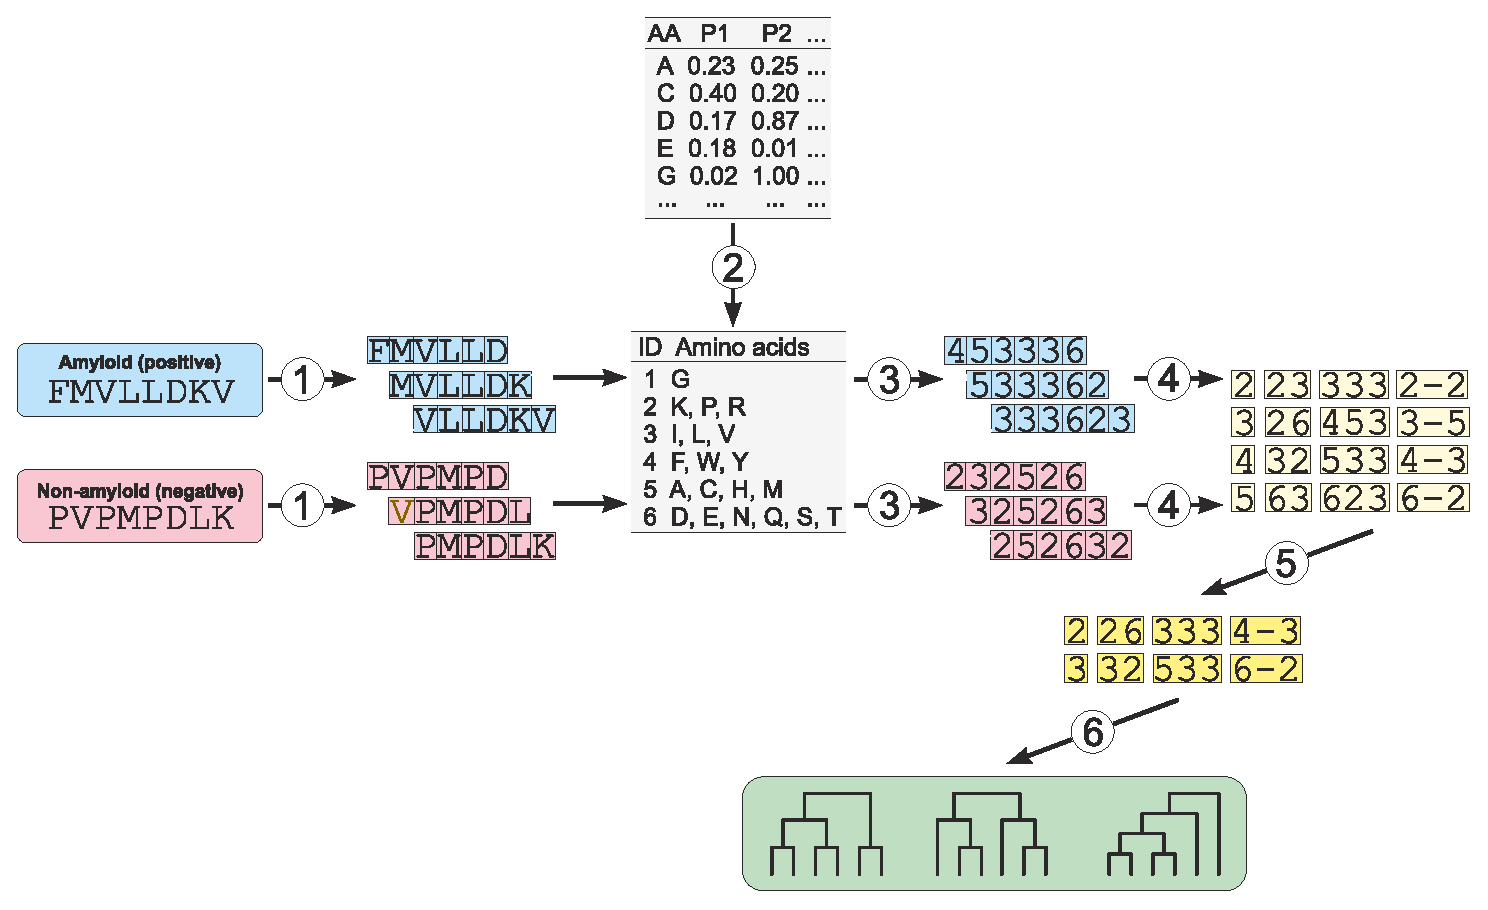
\includegraphics[width=0.95\textwidth]{static_figure/scheme.eps}
\end{figure}

3. Encoding amino acids of hexamers into corresponding groups (reduced alphabet). 
\end{frame}

    \begin{frame}{}
\begin{figure} 
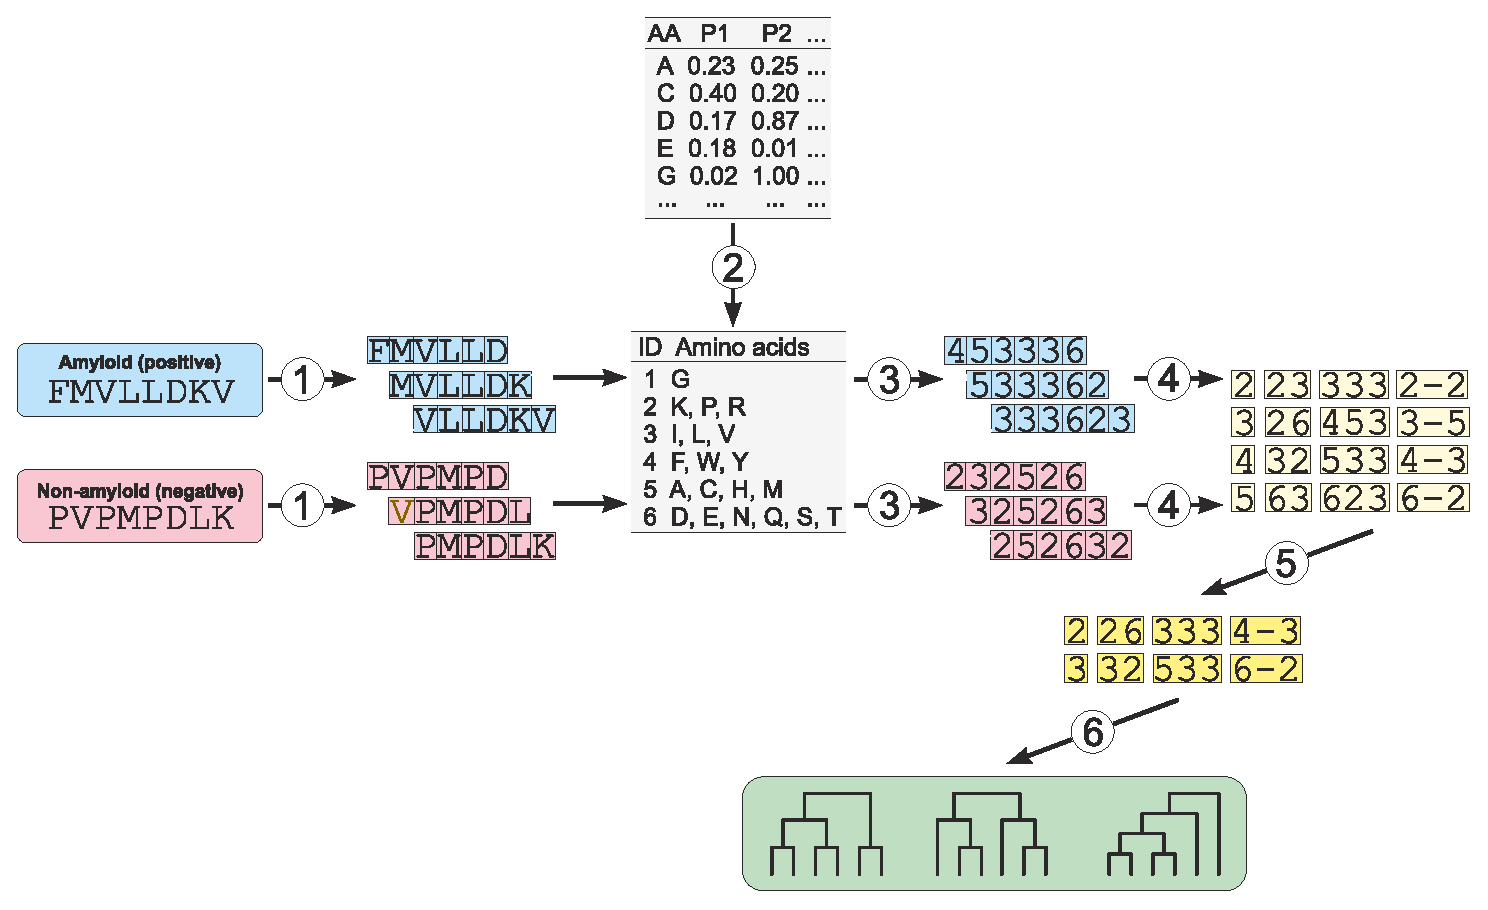
\includegraphics[width=0.95\textwidth]{static_figure/scheme.eps}
\end{figure}

4. Extraction of encoded n-grams of different types.
\end{frame}

  \begin{frame}{}
\begin{figure} 
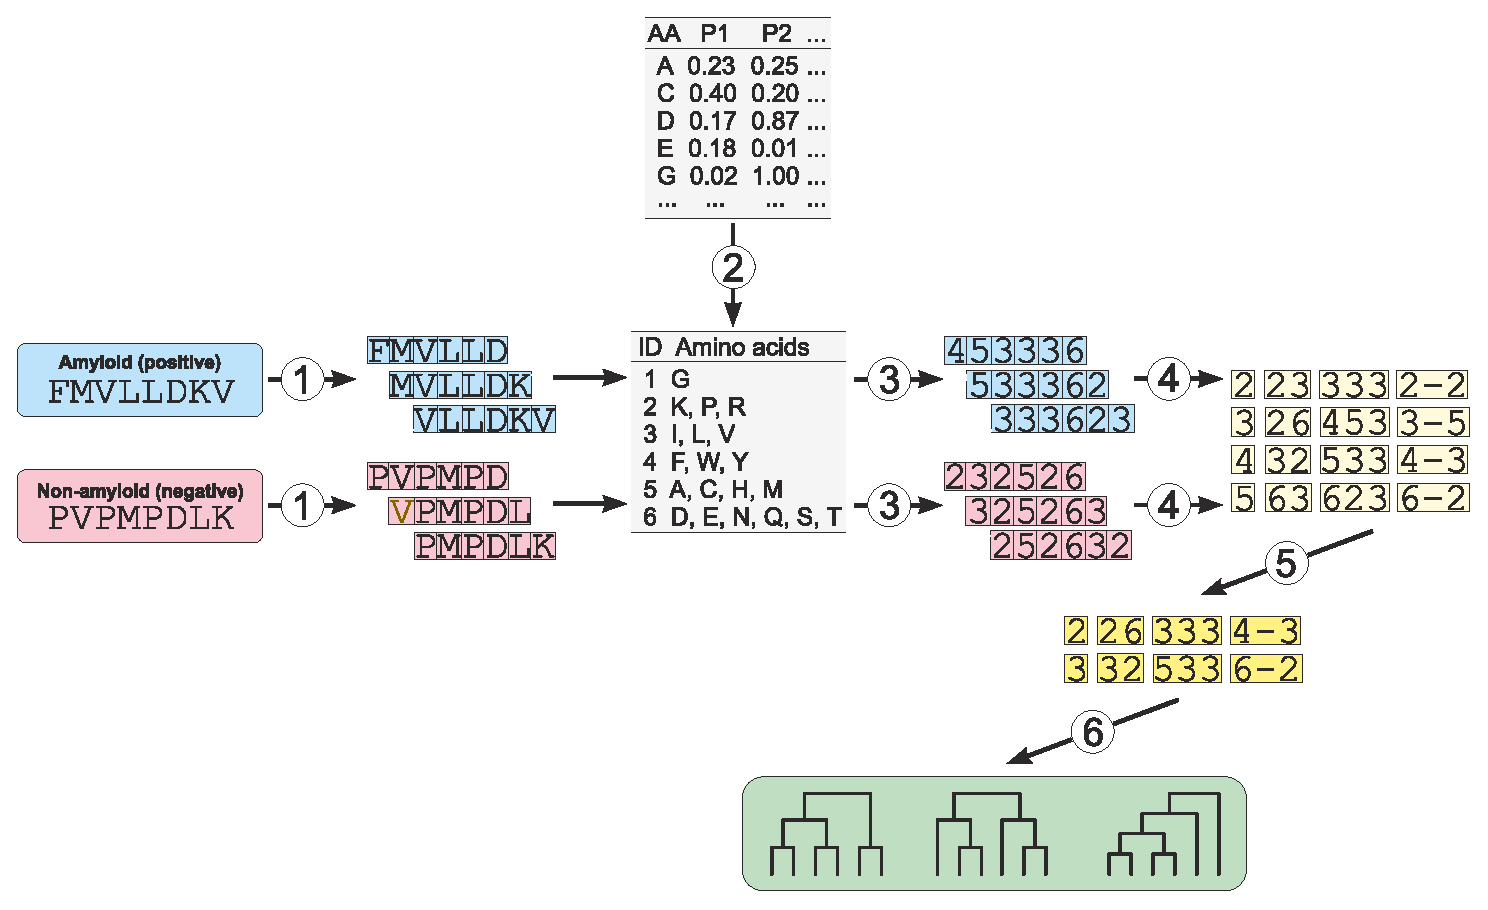
\includegraphics[width=0.95\textwidth]{static_figure/scheme.eps}
\end{figure}

5. Selection of informative n-grams using Quick Permutation Test (QuiPT).
\end{frame}

  \begin{frame}{}
\begin{figure} 
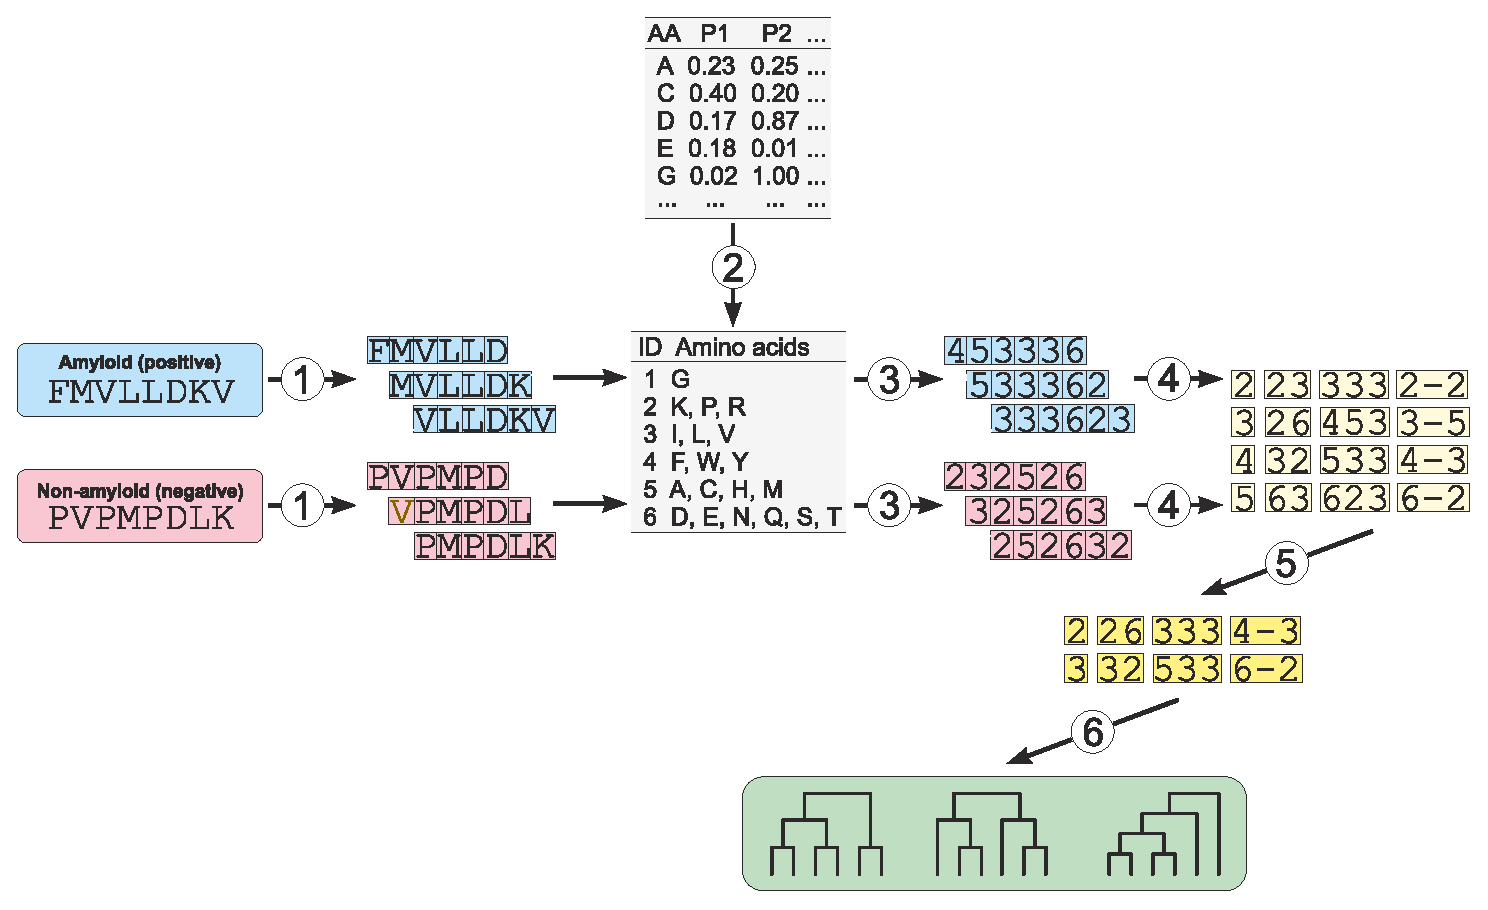
\includegraphics[width=0.95\textwidth]{static_figure/scheme.eps}
\end{figure}

6. Cross-validation of encodings using random forest classifier, which is trained on the informative n-grams.
\end{frame}


%       \begin{frame}{}
% \begin{figure} 
% 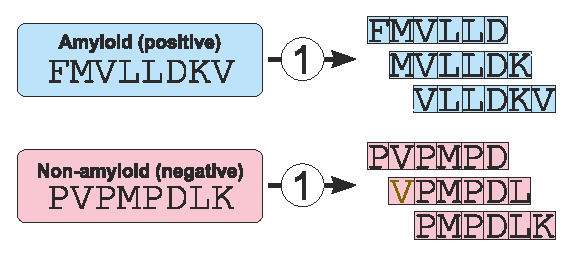
\includegraphics[width=0.55\textwidth]{static_figure/scheme1.eps}
% \end{figure}
% 
%   \end{frame}
  
  
%       \begin{frame}{Reduced amino acid alphabets}
% \begin{figure} 
% 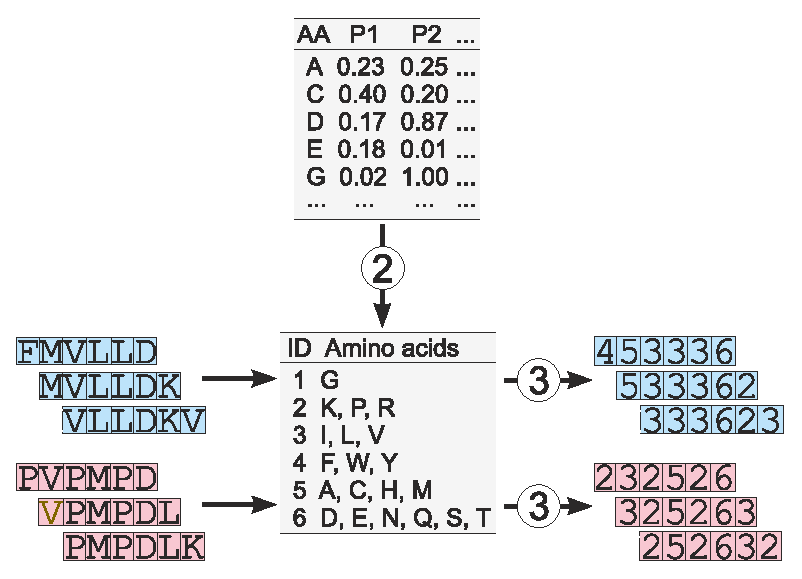
\includegraphics[width=0.75\textwidth]{static_figure/scheme2.eps}
% \end{figure}
% 
%   \end{frame}
  
  \begin{frame}{Reduced amino acid alphabets}

\begin{itemize}
\item 17 measures handpicked from AAIndex database 
  \begin{itemize}
    \item size of residues, 
    \item hydrophobicity, 
    \item solvent surface area, 
    \item frequency in $\beta$-sheets,
    \item contactivity.
  \end{itemize}
  \item 524 284 amino acid reduced alphabets with different level of amino acid alphabet reduction (three to six amino acid groups).
  \end{itemize}

    \end{frame}
  
  
%   \begin{frame}{Filtering n-grams}
% \begin{figure} 
% 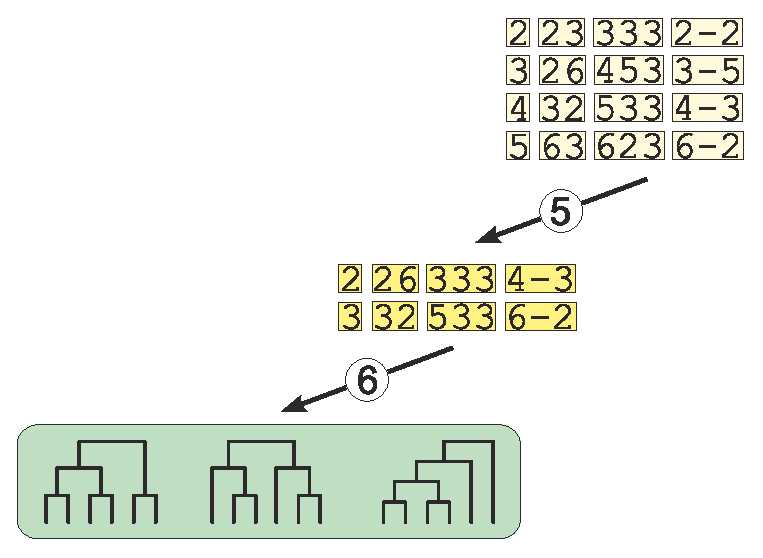
\includegraphics[width=0.65\textwidth]{static_figure/scheme3.eps}
% \end{figure}
% 
%   \end{frame}
  
  \begin{frame}{Quick Permutation Test}
  Informative n-grams are usually selected using permutation tests.

During a permutation test we shuffle randomly class labels and compute a defined statistic (e.g. information gain). Values of statistic for permuted data are compared with the value of statistic for original data.

$$
\textrm{p-value} = \frac{N_{T_P > T_R}}{N} $$

$N_{T_P > T_R}$: number of cases, where $T_P$ (permuted test statistic) has more extreme values than $T_R$ (test statistic for original data).

$N$: number of permutations.
  \end{frame}
  
\begin{frame}{QuiPT}  
  
  \textbf{Qui}ck \textbf{P}ermutation \textbf{T}est is a fast alternative to permutation tests for n-gram data. It also allows precise estimation of p-value.

QuiPT is avaible as part of the \textbf{biogram} R package.
\end{frame}
  
      
\section{Results}
  
    \begin{frame}{Cross-validation}
\begin{knitrout}
\definecolor{shadecolor}{rgb}{0.969, 0.969, 0.969}\color{fgcolor}

{\centering 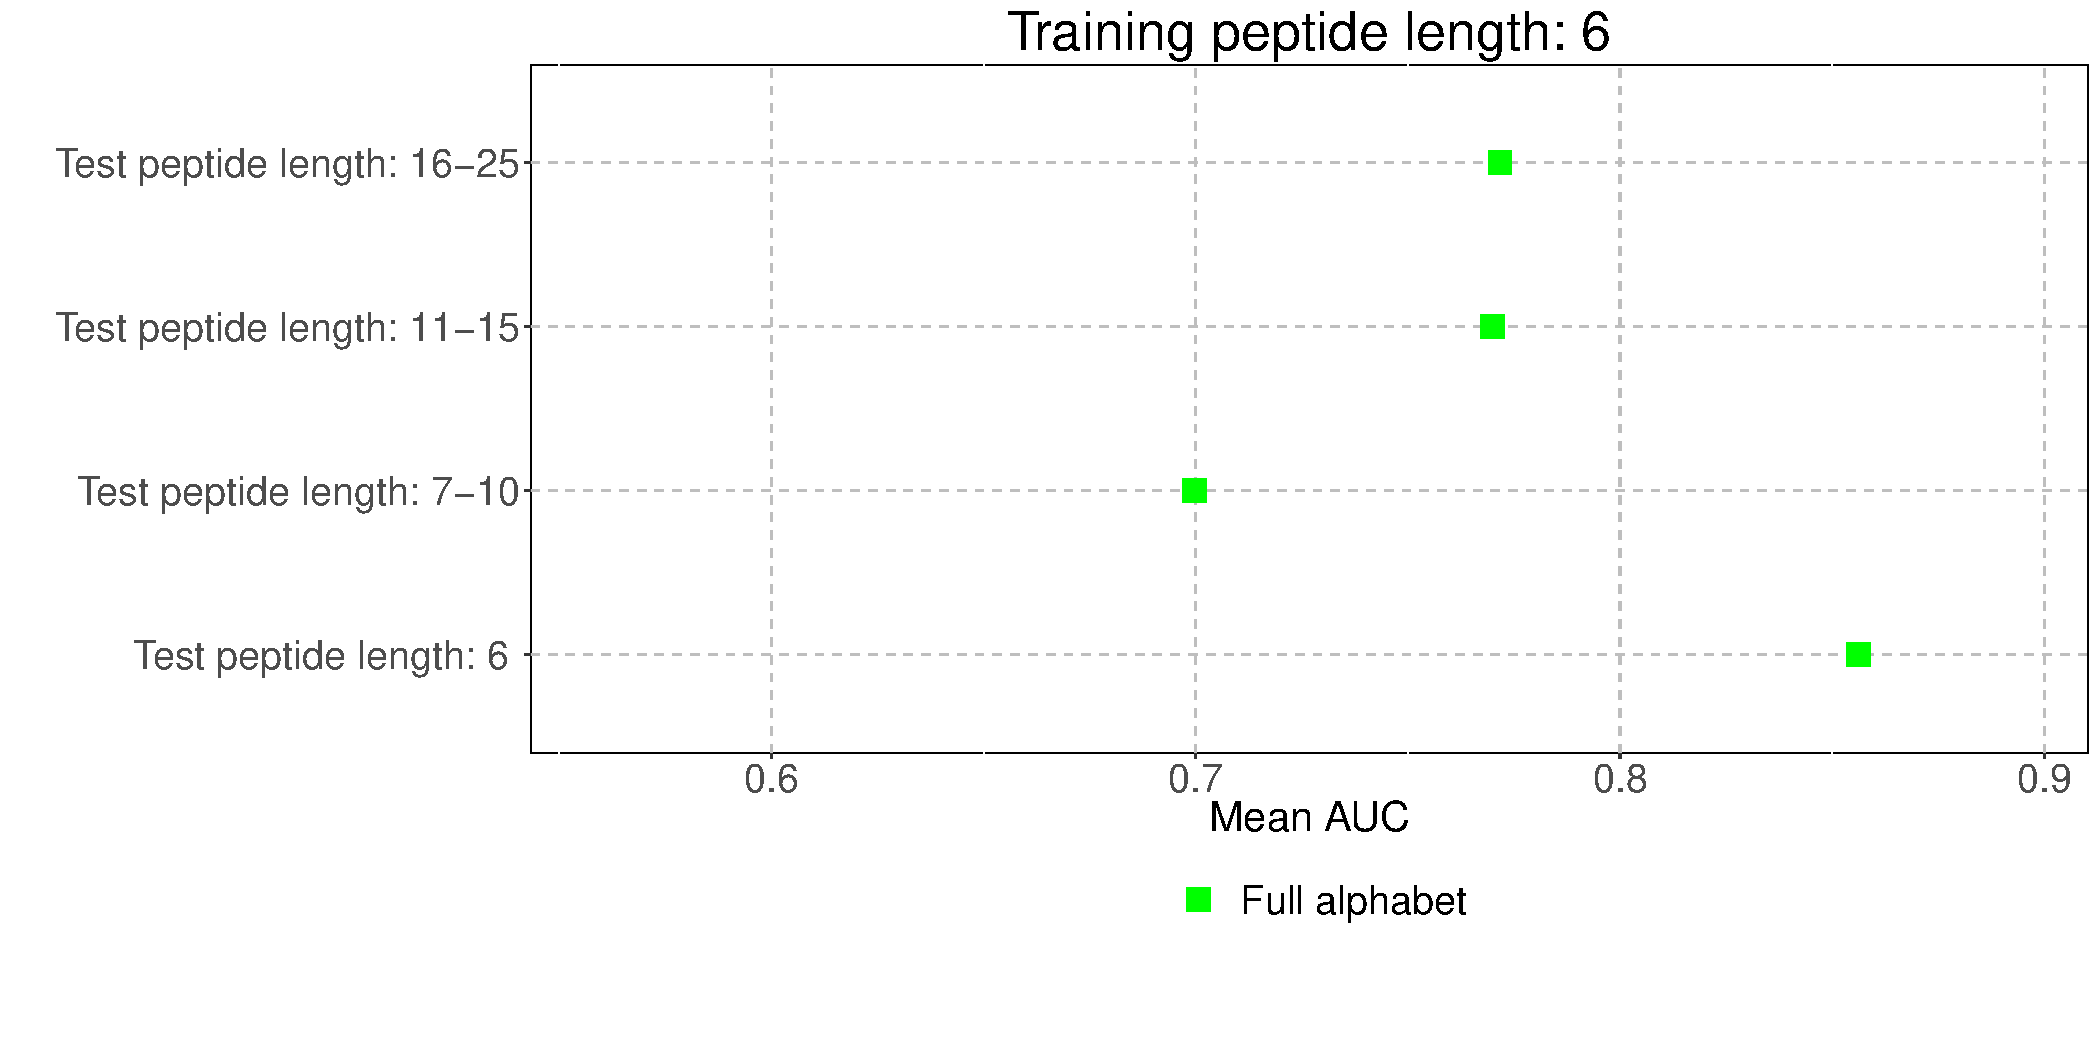
\includegraphics[width=\maxwidth]{figure/unnamed-chunk-1-1} 

}



\end{knitrout}
  
  \tiny
Hinges of boxes correspond to 
the 0.25 and 0.75 quartiles. The bar inside the box represents the median. The 
gray circles correspond to the reduced alphabets with the AUC outside the 0.95 
confidence interval.

  
  \end{frame}
  
    \begin{frame}{Cross-validation}
\begin{knitrout}
\definecolor{shadecolor}{rgb}{0.969, 0.969, 0.969}\color{fgcolor}

{\centering 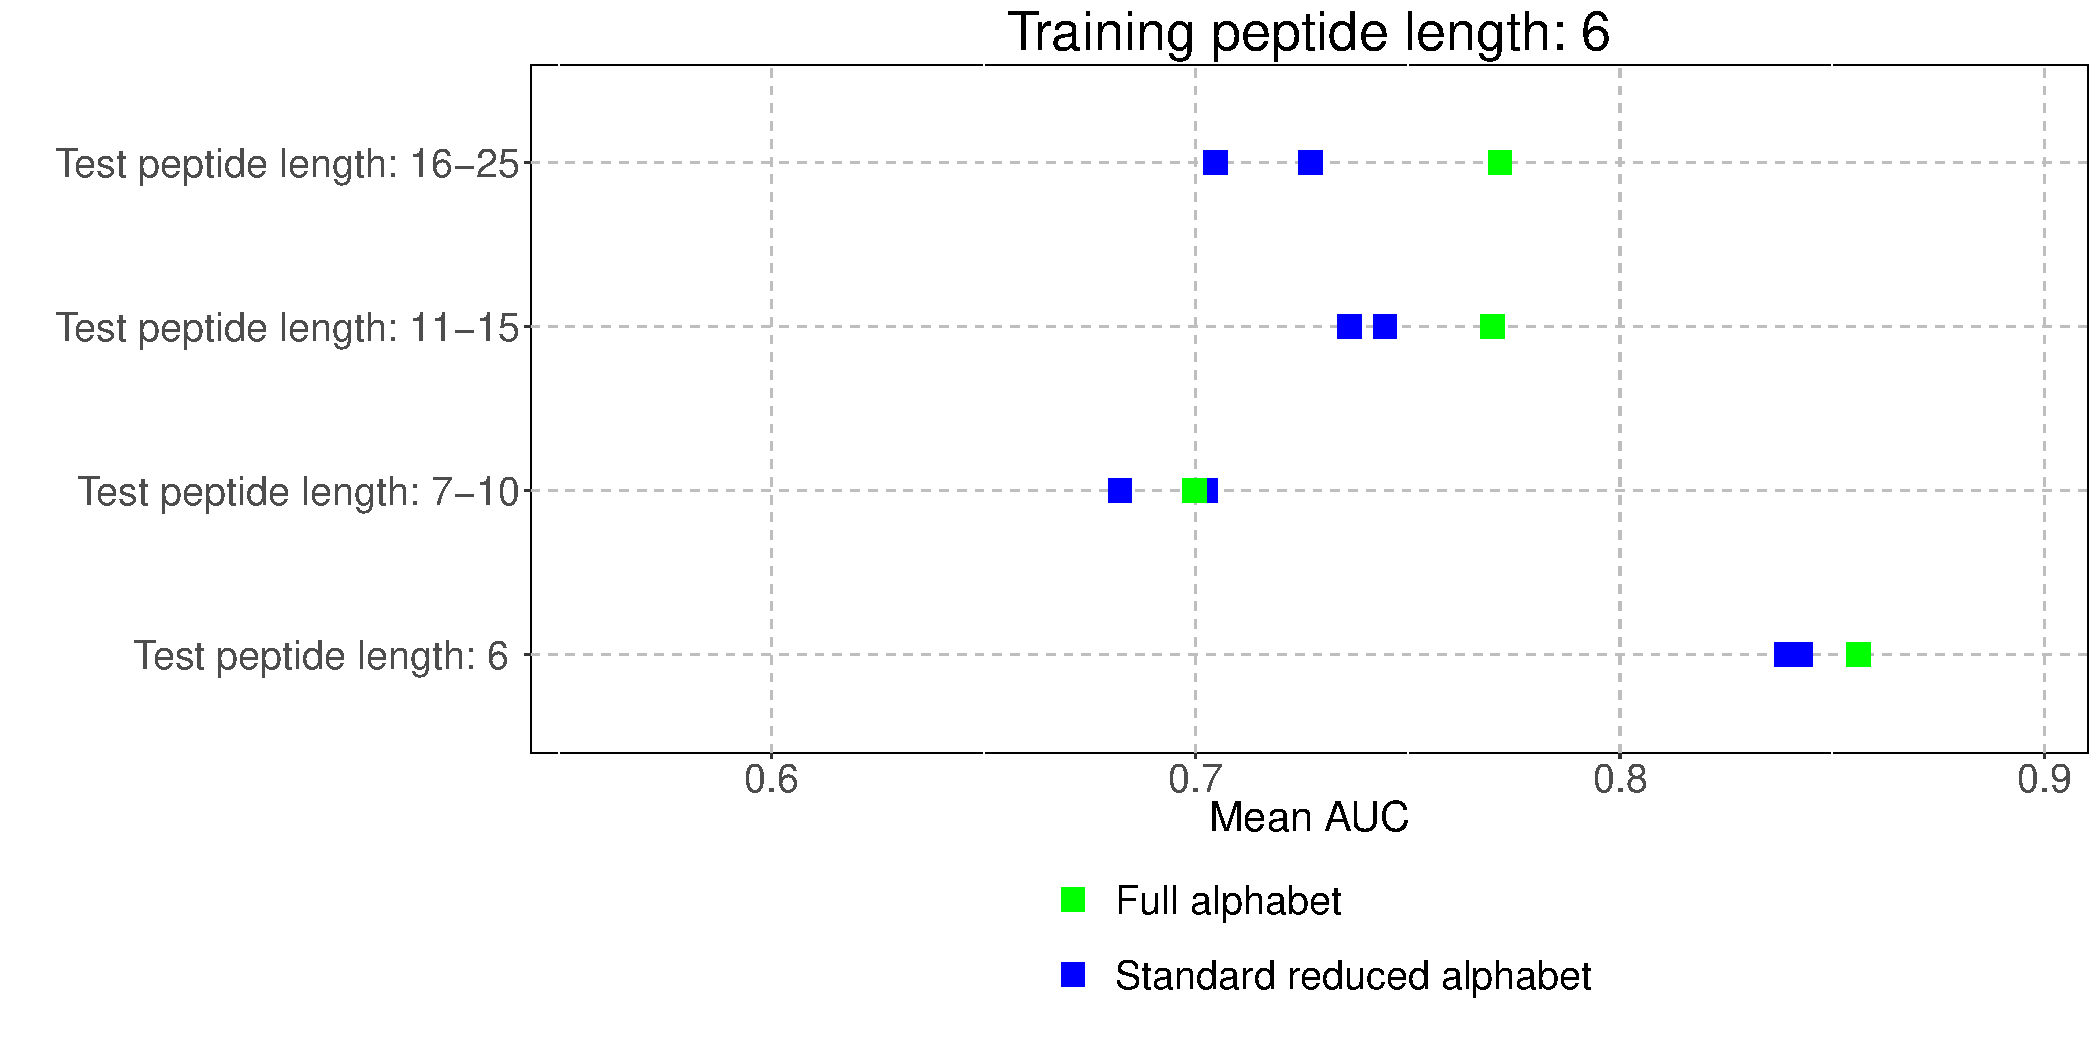
\includegraphics[width=\maxwidth]{figure/unnamed-chunk-2-1} 

}



\end{knitrout}
  \tiny
Hinges of boxes correspond to 
the 0.25 and 0.75 quartiles. The bar inside the box represents the median. The 
gray circles correspond to the reduced alphabets with the AUC outside the 0.95 
confidence interval.

  \end{frame}

%'     \begin{frame}{}
%'   <<echo = FALSE, message=FALSE,warning=FALSE,fig.align='center',fig.width=14,fig.height=7>>=
%' subdat <- filter(amyloids_plot, pos == "Training peptide length: 6-15")
%' 
%' ggplot(subdat, aes(x = len_range, y = AUC_mean)) +
%'   geom_boxplot(outlier.color = "grey", outlier.shape = 16, outlier.size = 5) +
%'   geom_point(data = filter(subdat, et != "Reduced alphabet"), 
%'              aes(x = len_range, y = AUC_mean, color = et, shape = et), size = 5) +
%'   scale_x_discrete("") +
%'   scale_y_continuous("Mean AUC") +
%'   scale_shape_manual("", values = c(16, 16, 15, 15), drop = FALSE) +
%'   scale_color_manual("", values = c("red", "grey", "green", "blue"), drop = FALSE) +
%'   guides(color = guide_legend(nrow = 2), shape = guide_legend(nrow = 2)) + 
%'   #facet_wrap(~ pos, nrow = 3) +
%'   ggtitle("Training peptide length: 6-15") + 
%'   my_theme + 
%'   coord_flip()
%' 
%' 
%' @
%'   \end{frame}  


\begin{frame}{}
Is the best-performing reduced amino alphabet associated with amyloidogenicity?
\end{frame}

\begin{frame}{Similarity index}
\begin{knitrout}
\definecolor{shadecolor}{rgb}{0.969, 0.969, 0.969}\color{fgcolor}

{\centering 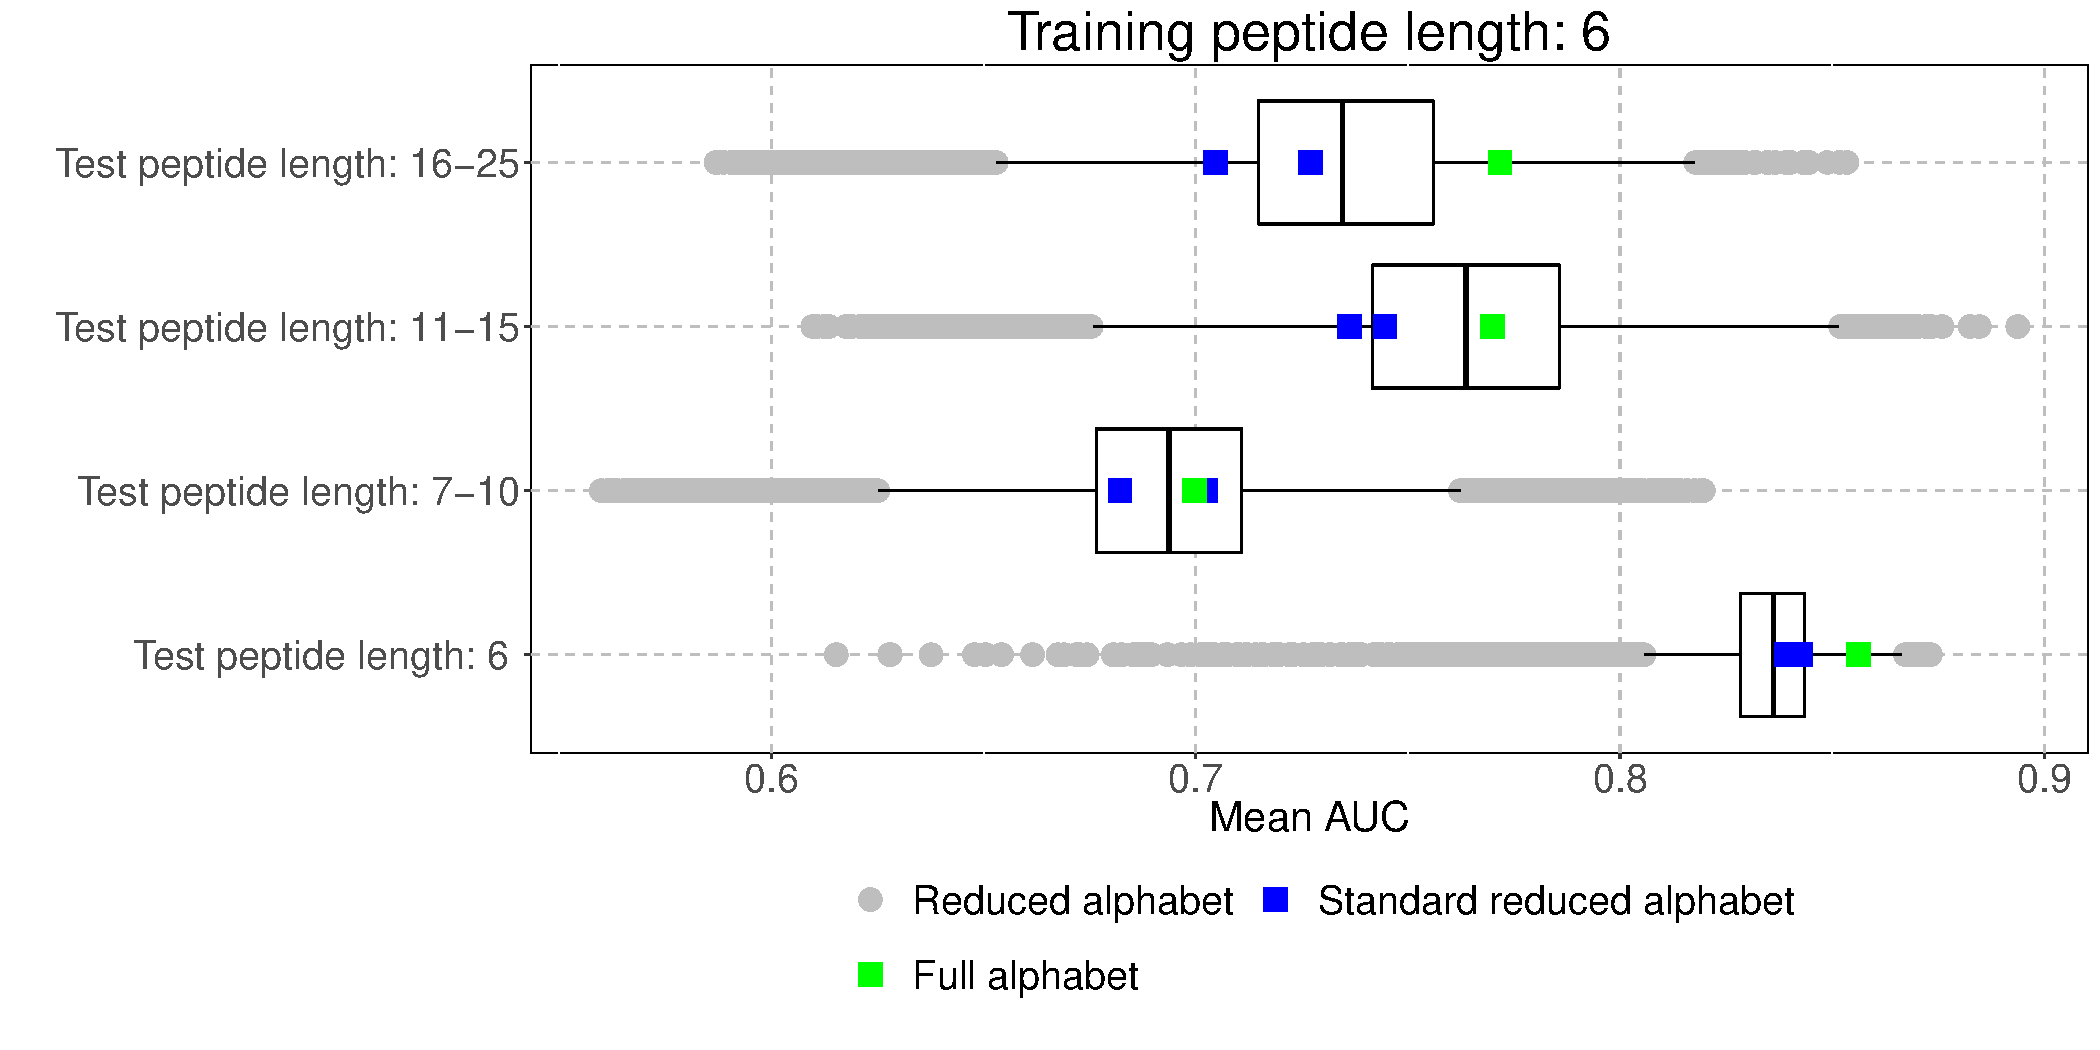
\includegraphics[width=\maxwidth]{figure/unnamed-chunk-3-1} 

}



\end{knitrout}
Similarity index~\citep{stephenson_unearthing_2013} measures the similarity between two reduced alphabets (1 - identical, 0, totally dissimilar).
\end{frame}

\begin{frame}{}
Are informative n-grams found by QuiPT associated with amyloidogenicity?
\end{frame}


\begin{frame}{Informative n-grams}
\begin{knitrout}
\definecolor{shadecolor}{rgb}{0.969, 0.969, 0.969}\color{fgcolor}

{\centering 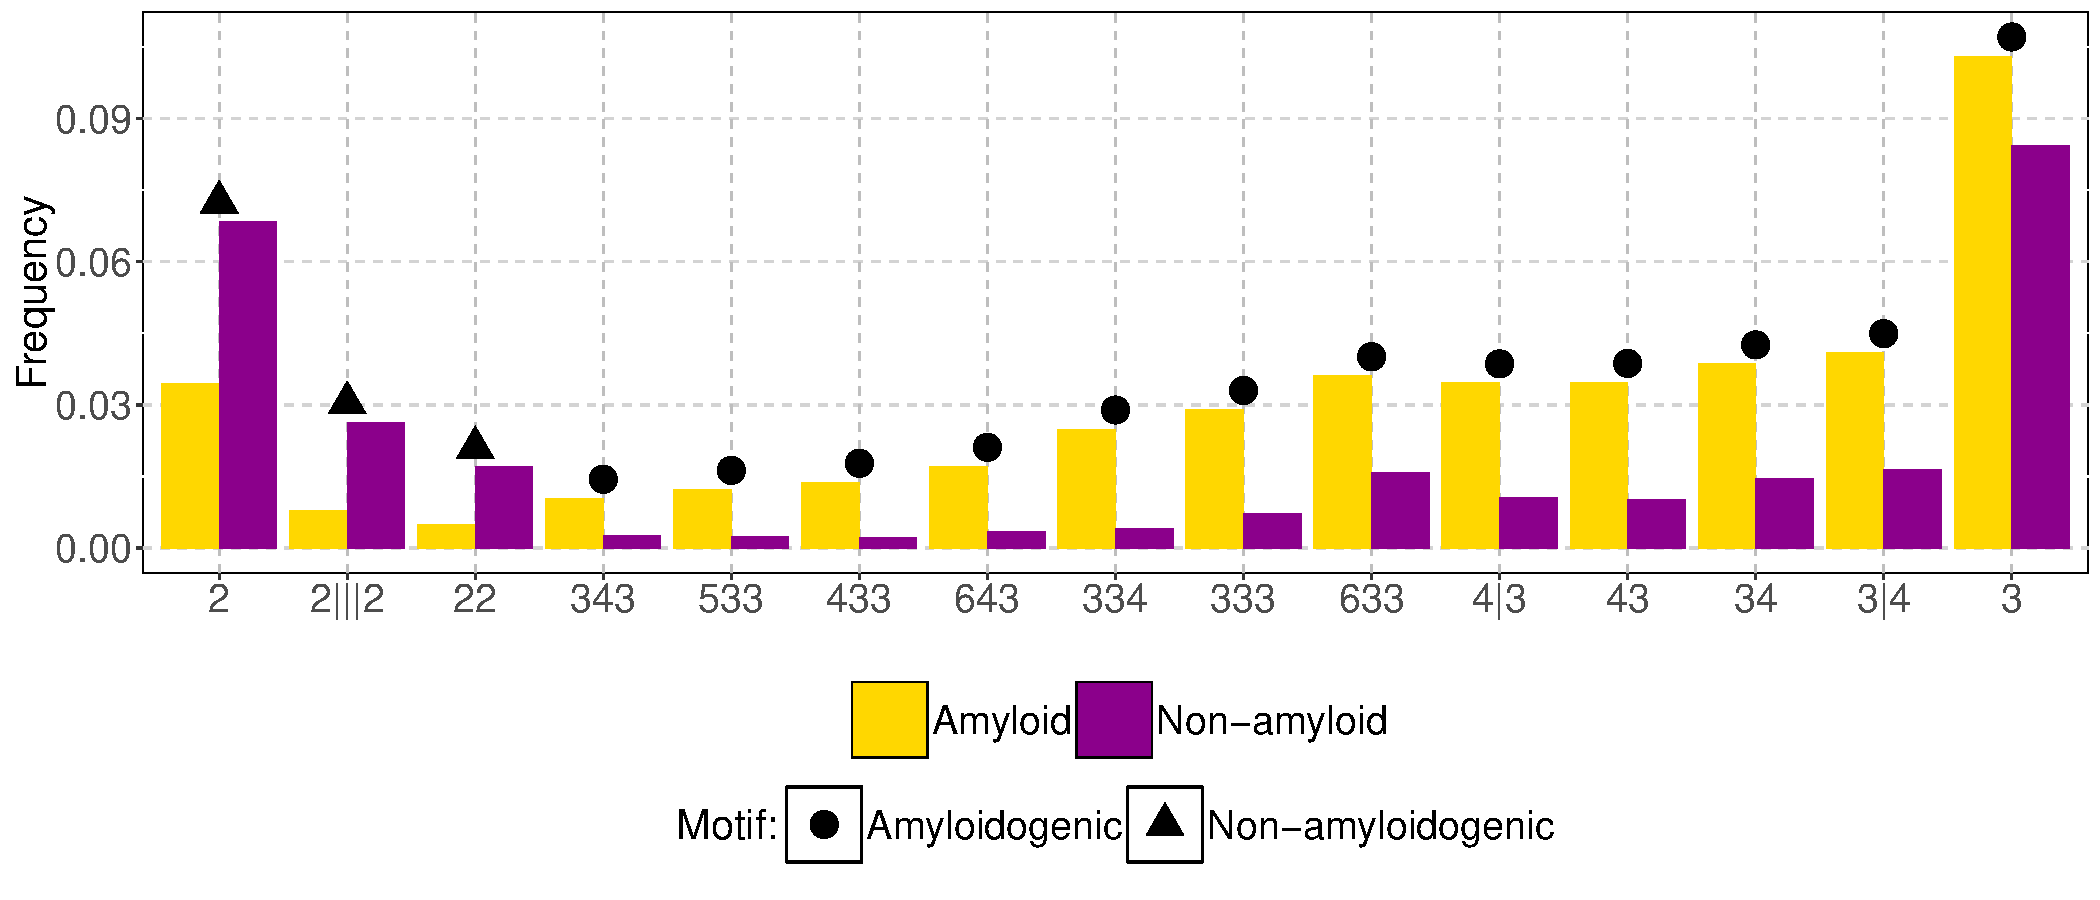
\includegraphics[width=\maxwidth]{figure/unnamed-chunk-4-1} 

}



\end{knitrout}

Out of 65 the most informative n-grams, 15 (23\%) were also found in the motifs validated experimentally~\citep{paz_sequence_2004}.
\end{frame}

\begin{frame}{}
Is performance of the AmyloGram, the classifier based on the best-performing reduced amino acid alphabet, also adequate on the independent dataset?
\end{frame}


\begin{frame}{Benchmark results}

\begin{table}[ht]
\centering

\begin{tabular}{ccccc}
  \toprule
Classifier & AUC & MCC \\ 
  \midrule
AmyloGram & \textbf{0.8972} & \textbf{0.6307} \\ 
  \rowcolor{white}PASTA 2.0\citep{walsh_pasta_2014} & 0.8550 & 0.4291  \\ 
   FoldAmyloid \citep{garbuzynskiy_foldamyloid:_2010} & 0.7351 & 0.4526  \\ 
  \rowcolor{white}APPNN \citep{familia_prediction_2015} & 0.8343 & 0.5823  \\ 
   \bottomrule
\end{tabular}
\end{table}

The predictor based on the best-performing alphabet, called AmyloGram, was benchmarked against the most popular tools for the detection of amyloid peptides using an external data set \textit{pep424}.

\end{frame}

\begin{frame}{Summary}

We identified a group of reduced amino acid alphabets which capture properties of amyloids. 

Our algorithm was also capable of extracting n-gram associated with amyloidogenicity, partially confirming experimental results.

Our software is available as a web-server: \url{smorfland.uni.wroc.pl/amylogram}.

\end{frame}

\begin{frame}{Funding}

This research was partially funded by the KNOW Consortium and National Science Center (2015/17/N/NZ2/01845).

\end{frame}



\begin{frame}[allowframebreaks]
        \frametitle{References}
  \bibliographystyle{apalike}
  \bibliography{references}
\end{frame}  
\end{document}
